\documentclass[12pt]{article}
\usepackage{amsmath}
\usepackage{enumerate}
\usepackage{mathrsfs} 
\usepackage{amsthm}
\usepackage{amsfonts}
\usepackage{amssymb}
\usepackage{latexsym} 
%\usepackage{epsfig}
%\usepackage{graphicx}
%\usepackage[dvips]{graphicx}
\usepackage{tikz}
\usepackage{tikz-cd}



\usepackage[matrix,tips,graph,curve]{xy}

\newcommand{\mnote}[1]{${}^*$\marginpar{\footnotesize ${}^*$#1}}
\linespread{1.065}

\makeatletter

\setlength\@tempdima  {5.5in}
\addtolength\@tempdima {-\textwidth}
\addtolength\hoffset{-0.5\@tempdima}
\setlength{\textwidth}{5.5in}
\setlength{\textheight}{8.75in}
\addtolength\voffset{-0.625in}

\makeatother

\makeatletter 
\@addtoreset{equation}{section}
\makeatother


\renewcommand{\theequation}{\thesection.\arabic{equation}}

\theoremstyle{plain}
\newtheorem{theorem}[equation]{Theorem}
\newtheorem{corollary}[equation]{Corollary}
\newtheorem{lemma}[equation]{Lemma}
\newtheorem{proposition}[equation]{Proposition}
\theoremstyle{definition}
\newtheorem{definition}[equation]{Definition}
\newtheorem{definitions}[equation]{Definitions}
%\theoremstyle{remark}

\newtheorem{remark}[equation]{Remark}
\newtheorem{remarks}[equation]{Remarks}
\newtheorem{exercise}[equation]{Exercise}
\newtheorem{example}[equation]{Example}
\newtheorem{examples}[equation]{Examples}
\newtheorem{notation}[equation]{Notation}
\newtheorem{question}[equation]{Question}
\newtheorem{assumption}[equation]{Assumption}
\newtheorem*{claim}{Claim}
\newtheorem{answer}[equation]{Answer}
%%%%%% letters %%%%

\newcommand{\fa}{\mathfrak{a}}
\newcommand{\fb}{\mathfrak{b}}
\newcommand{\fm}{\mathfrak{m}}
\newcommand{\fp}{\mathfrak{p}}
\newcommand{\fq}{\mathfrak{q}}

\newcommand{\IA}{\mathbb{A}}
\newcommand{\IN}{\mathbb{N}}
\newcommand{\IP}{\mathbb{P}}
\newcommand{\IZ}{\mathbb{Z}}

\newcommand{\sO}{\mathcal{O}}

\newcommand{\shF}{\mathscr{F}}
\newcommand{\shG}{\mathscr{G}}
%%%%%%% macros %%%%%

%% my definitions %%%

\newcommand{\End}{\mathrm{End}}
\newcommand{\tr}{\mathrm{tr}}
\newcommand{\Hom}{\mathrm{Hom}}
\newcommand{\Aut}{\mathrm{Aut}}
\newcommand{\Trace}{\mathrm{Trace}\,}
\newcommand{\rank}{\mathrm{rank}}
\renewcommand{\deg}{\mathrm{deg}\,}
\newcommand{\Spec}{\rm Spec\,}
\newcommand{\Sym}{\mathrm{Sym \,}}
\newcommand{\Span}{\mathrm{Span \,}}
\renewcommand\dim{{\rm dim\,}}
\renewcommand\det{{\rm det\,}}
\newcommand{\sing}{{\rm sing}}


\newcommand\iso{{\, \cong \,}} 
\newcommand\tensor{{\otimes}}
\newcommand\Tensor{{\bigotimes}} 
\newcommand\union{\bigcup} 
\newcommand\onehalf{\frac{1}{2}}
\newcommand\trivial{{\mathbb I}}
\newcommand\wb{\overline}

%%%%%Delimiters%%%%

\newcommand{\<}{\langle}
\renewcommand{\>}{\rangle}

%\renewcommand{\(}{\left(}
%\renewcommand{\)}{\right)}


%%%% Different kind of derivatives %%%%%

\newcommand{\delbar}{\bar{\partial}}
\newcommand{\pdu}{\frac{\partial}{\partial u}}
%\newcommand{\pd}[1][2]{\frac{\partial #1}{\partial #2}}

%%%%% Arrows %%%%%
\newcommand{\induce}{\rightsquigarrow}
\newcommand{\into}{\hookrightarrow}
\newcommand{\onto}{doubleheadarrow}
\newcommand{\tto}{\longmapsto}
\def\llra{\longleftrightarrow}
\def\wt{\widetilde}
\def\wtilde{\widetilde}
\def\what{\widehat}
\def\bf{\textbf}
\def\it{\textit}
%%%%%%%%%%%%%%%%%%% Ziquan's definitions %%%%%%%%%%%%%%%%%%%%
\newcommand{\Ann}{\mathrm{Ann}}
\newcommand{\height}{\mathrm{height \,}}
\newcommand{\Div}{\mathrm{Div}}
\newcommand{\sE}{\mathcal{E}}
\newcommand{\p}{\partial}
%%%%%%%%%%%%% new definitions for the positive mass paper %%%%%%%%%

\newcommand{\sperp}{{\scriptscriptstyle \perp}}
\newcommand{\st}{\mathrm{s.t.}\,}

%%%%%%%%%%%%%%%%%%%%%%%

%%%%%%%%%%%%%%%%%%%%%%%%%%%%%%%%%%%%%%%%%%%%%



%
\begin{document}
%

\title{Elliptic Surfaces}
\author{Ziquan Yang}


\date{May 14, 2015}

\maketitle
 
%\setcounter{secnumdepth}{1} 

\setcounter{section}{0}

\section{Introduction}
Consider hypersurfaces in $\IP^2 \times \IP^1$ of bidegree $(3, d)$. These hypersurfaces are parametrized by $P = \IP V$, where
$$ V = H^0 ( \IP^2 \times \IP^1, \sO(3, d) ) $$
Let $P^0$ be the subscheme parametrizing those non-singular ones:
$$ P^0 = \{ f \in P : H_f \textit{ is non-singular }\} $$
Let $\pi : \IP^2 \times \IP^1 \to \IP^1$ be projection to the second component. If $H_f$ is non-singular, then fibers of $\pi|_{H_f}$ are cubic curves in $\IP^2$. This makes $H_f$ an elliptic surface. The analogy of being simply ramified for $H_f$ has to do with singular fibers of the map $\pi : H_f \to \IP^1$. Smooth fibers are all isomorphic to the smooth cubic curve. It is customary for some literature to call an irredcucible cubic curve, together with a specified point as the base point, an elliptic curve. There are many types of singular fibers. If the fiber is irreducible, then it is either a nodal curve (e.g. $y^2 = x^2 - x^3$), or a cuspidal curve (e.g. $y^2 = x^3$). If the fiber is not irreducible, then it may be a union of a conic curve and a line, or a union of three lines and there are many different configurations of irreducible components. 
An analogue of a simply ramified curve would be a hypersurface whose singular fibers are all nodal curves. Why is an analogue would be clear in the discussion of Euler characteristics. Hence we are primarily concerned with the following subset of $P^0$: 
$$ D = \{ f \in P^0 : \textit{all singular fibers of $H_f$ are nodal curves} \}$$

For future use we introduce some notation. Let $X$ be a scheme and $f : X \to Y$ be a morphism. For $P \in Y$, we denote the fiber $f^{-1}(P)$ by $X_P$ when $f$ is clear in the context. We denote the singular locus of $X$ by $X_\sing$. If $X \subseteq \IP^n$ and $Q \in \IP^n$, we denote the tangent cone of $X$ at $Q$ by $TC_Q(X)$. If $Q \not\in X$, then $TC_Q(X) = \IP^n$. 

\section{Euler Characteristic}
Just like the genus of a curve tells us the degree of the ramification divisor for a curve of bidegree $(n, d)$ in $\IP^1 \times \IP^1$, the Euler characteristic of a hypersurface in $\IP^2 \times \IP^1$ tells us something about singular fibers. Let $f \in P^0$ and $H_f$ be the corresponding hypersurface. With respect to the map $\pi : H_f \to \IP^1$ we may write $X$ as $X^0 \coprod C$, where $C$ is the finite set of points with singular fibers and $X^0$ is its complement, and $Y$ as $Y^0 \coprod \pi^{-1}(C)$, where $Y^0 = \pi^{-1} X^0$. Let $F$ be the smooth cubic curve in $\IP^2$, we see that $Y^0$ is a $F$-bundle of $X^0$, and their Euler characteristics are related by 
$$ e(Y^0) = e(X^0 ) \cdot e(F) $$ 
Since $e(F) = 0$ we have that $e(Y^0) = 0$. Now since $Y = Y^0 \coprod \pi^{-1}(C)$, we see that $e(Y) = e(Y^0) + e(\pi^{-1}(C)) = e(\pi^{-1}(C))$. Note that $C$ is a finite set of points, and hence $\pi^{-1} (C)$ is a disjoint union of singular cubic curves. 

\begin{figure}[h!]
  \centering
      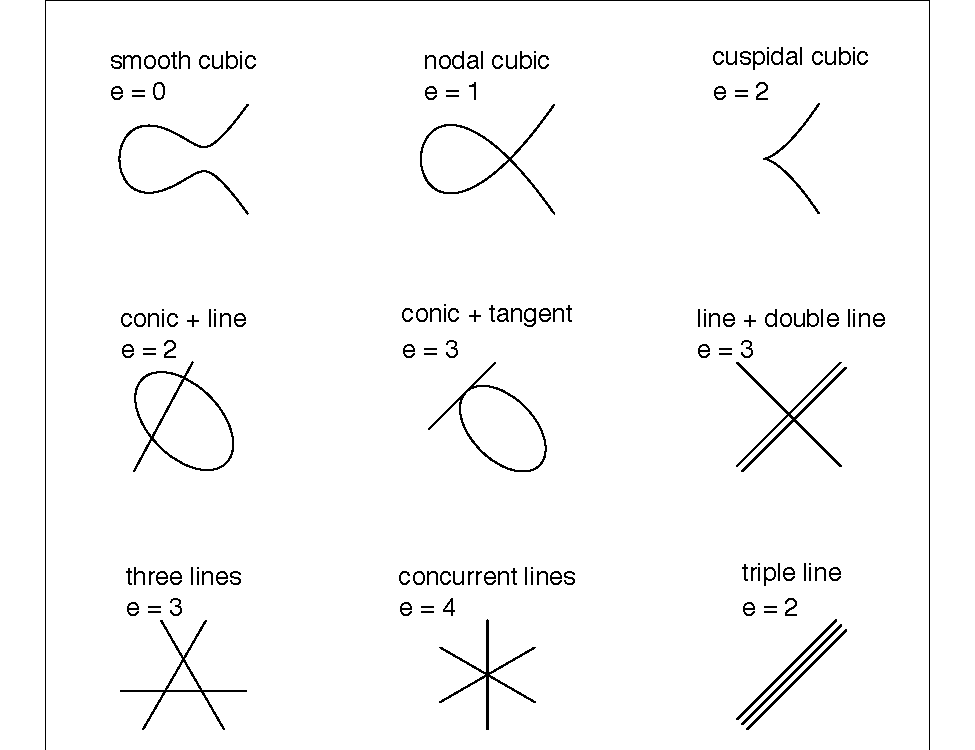
\includegraphics[width=1.0\textwidth]{planecubics}
  \caption{Cubic plane curves and their Euler characteristics \cite{Pic}}
\end{figure}
From the table we see that if $f \in D$, then $e(H_f)$ is exactly the number of points in $\IP^1$ over which the fibers are singular. In this sense, these hypersurfaces are analogues of simply ramified curves in $\IP^1 \times \IP^1$. 

Now we compute $e(H_f)$. In fact we do a more general computation, since it is not harder. Let $H_f \subseteq \IP^2 \times \IP^1$ be a smooth hypersurface of bidegree $(n, d)$. We denote the projections of $\IP^2 \times \IP^1$ onto the first and second components by $\pi_1, \pi_2$ respectively. Let $H_1$ be a hyperplane of $\IP^2$ and $H_2$ be a hyperplane of $\IP^1$. We think of them as generators of the Chow groups of their respective projective schemes. We define 
$$ A = \pi_1^*(H_1), \, E = \pi_2^*(H_2) $$
and $$ h_1 = A \cap H_f, \, h_2 = E \cap H_f $$
We compute the Chern classes of $H_f$ using the standard exact sequence:
$$ 0 \to T_{H_f} \to T_{\IP^2 \times \IP^1|_{H_f}} \to N_{H_f/\IP^2 \times \IP^1} \to 0$$
By Whitney\rq{}s formula, their total Chern classes are related by
$$ c(T_{\IP^2 \times \IP^1|_{H_f}}) = c(T_{H_f}) c(N_{H_f/\IP^2 \times \IP^1}) $$
Now $T_{\IP^2 \times \IP^1|_{H_f}}$ is $T_{\IP^2 \times \IP^1} = \pi_1^* T_{\IP^2} \oplus \pi_2^* T_{\IP^1}$ restricted to $H_f$, so we obtain 
$$ c(T_{\IP^2 \times \IP^1|_{H_f}}) = (1 + 3h_1 + 3h_1^2)(1 + 2h_2) $$
If $\iota : H_f \into \IP^2 \times \IP^1$ is the inclusion, then $$N_{H_f/\IP^2 \times \IP^1} = \iota^* \sO_{\IP^2 \times \IP^1}(nA  + dE) = (1 + nh_1 + dh_2)$$
Therefore 
\begin{align*}
c(T_{H_f}) &= c(T_{\IP^2 \times \IP^1|_{H_f}})c(N_{H_f/\IP^2 \times \IP^1})^{-1}\\
&= (1 + 3h_1 + 3h_1^2)(1 + 2h_2)(1 + nh_1 + dh_2)^{-1}\\
&= (1 + 3h_1 + 3h_1^2)(1 + 2h_2)(1 - (nh_1 + dh_2) + (nh_1 + dh_2)^2 - \cdots)
\end{align*}
In particular we obtain 
$$ c_2(T_{H_f}) = (n^2 - 3n + 3)h_1^2 + (6 + 2nd - 2n - 3d)h_1 h_2 $$
which is the top Chern class. Now we compute 
\begin{align*}
\deg h_1^2 &= A \cdot A \cdot (nA + dE) = d \\
\deg h_1 h_2 &= A \cdot E \cdot (nA + dE) = n 
\end{align*}
Finally we obtain 
$$ e(H_f) = \deg c_2(T_{H_f}) = 6n + 3d + 3n^2 d - 6 dn - 2n^2 $$
In particular, for future use we want to fix $n = 3$, so $e(H_f)$ depends only on $d$. In this case $e(H_f) = 12 d$.  

\section{An Analogue of Bertini\rq{}s Theorem}
Let $k$ be algebraically closed. We show an analogue of Bertini's theorem: 
\begin{theorem}
$D$ is a constructible subset of $\IP V$, and $D \neq \IP V$. 
\end{theorem}
Let $X = \IP^2 \times \IP^1$. In this section by ``fiber" the underlying morphism is always the projection $\pi : X \to \IP^1$, or its restrictions. We define 
$$ R = \{ f \in \IP V : \exists P \in \IP^1, \st (H_f)_P \textit{ is reducible} \} $$
and 
$$ C = \{ f \in \IP V : \exists P \in \IP^1, Q \in X_P, \st Q \in ((H_f)_P)_\sing \textit{ and } TC_Q((H_f)_P) \textit{ is a line}\}$$
Note that $C - R$ parametrizes those hypersurfaces $H_f$ that have some singular fiber isomorphic to a cuspidal curve. Therefore if $D' = \IP V - R \cup C$, then $D = D' \cap P^0$. It suffices to show that $R, C$ are both constructible, and $\dim R, \dim C < \dim \IP V$. 

\begin{lemma}
$R$ is constructible and $\dim R < \dim \IP V$. 
\end{lemma}
\begin{proof}
Let $\Delta$ be the image of the diagonal map $\IP^2 \to \IP^2 \times \IP^2$. Consider the scheme
$$ E = (\IP^2 \times \IP^2 - \Delta) \times \IP^1 \times \IP V$$ and let $\Pi : E \to \IP V$ be the projection to the last component. We want to define a subcheme $G \subseteq E$ parametrizing tuples $((P, Q), T, f)$ such that $(H_f)_T$ passes through $P, Q$ and the line $l$ in $\IP^2$ connecting $P, Q$ is an irreducible component of $(H_f)_T$. Then $\Pi(G) = R \subseteq \IP V$. Suppose $H_f$ is smooth and $(H_f)_T$ is a cubic plane curve. Bezout's theorem tells that if $(H_f)_T$ meets $l$ at $P, Q$, each with multiplicity $\ge 2$, then in fact $l \subseteq H_f$. We describe $G$ locally, but from the equations it is also not hard to give the equations that desribe $G$ globally. On an affine chart 
$$ (\IA^2 \times \IA^2 - \Delta) \times \IA^1 \subseteq (\IP^2 \times \IP^2 - \Delta) \times \IP^1 $$
we label the coordinates as 
$$ ((x_0, x_1), (y_0, y_1)), t)$$
Given $f \in V$, let $f_t = f(\cdot, t)$. We first describe $(x_0, x_1), (y_0, y_1) \in (H_f)_t$: 
$$f_t(x_0, x_1) = f_t(y_0, y_1) = 0$$
Then heuristically we want to require
$$ \frac{y_1 - x_1}{y_0 - x_0} = \frac{d x_1}{d x_0} = \frac{d y_1}{d y_0} $$
We can easily realize this by imposing two more equations: 
\begin{align*}
\frac{\p f_t}{\p y_0} (y_1 - x_1) = \frac{\p f_t}{\p y_1} (y_0 - x_0), \,
\frac{\p f_t}{\p x_0} (y_1 - x_1) = \frac{\p f_t}{\p x_1} (y_0 - x_0)
\end{align*}
If $f$ satisfies the above equations, then clearly so does any $af$ for $a \in k^*$. Therefore these equations are well defined for $f \in \IP V$ and describe $G \subseteq E$. To do dimension counting we factor $\Pi$ as $$ E \stackrel{p_1}{\to} \IP^1 \times \IP V \stackrel{p_2}{\to} \IP V $$
\end{proof}
Let $G'$ be the image of $p_1 : G \to \IP^1 \times \IP V$. By $G'_T$ we denote the fiber over $T \in \IP^1$ under the projection $\IP^1 \times \IP V \to \IP^1$. 



\begin{thebibliography}{9}
\bibitem{Pic}
B. Poonen, An explicit algebraic family of genus-one curves violating the Hasse principle, available at \textit{http://www-math.mit.edu/~poonen/}


\end{thebibliography}
                                                                                                                                                                                                                                                                                                                                                                                                                                                                                                                                                                                                                                                                                                                                                                                                                                                                                                                                                                                                                                                                                                                                                                                                                                                                                                                                                                                                                                                                                                                                                                                                                                                                                                                                                                                                                                                                                                                                                                                                                                                                                                                                                                                                                                                                                                                                                                                                                                                                                                                                                                                                                                                                                                                                                                                                                                                                                                                                                                                                                                                                                                                                                                                                                                                                                                                                                                                                                                                                                                                                                                                                                                                                                                                                                                                                                                                                                                                                                                                                                                                                                                                                                                                                                                                                                                                                                                                                                                                                                                                                                                                                                                                                                                                                                                                                                                                                                                                                                                                                                                                                                                                                                                                                                                                                                                                                                                                                                                                                                                                                                                                                                                                                                                                                                                                                                                                                                                                                                                                                                                                                                                                                                                                                                                                                                                                                                                                                                                                                                                                                                                                                                                                                                                                                                                                                                                                                                                                                                                                                                                                                                                                           


\end{document}